% Template for laboratory reports 
% Feel free to modify or redistribute this template,  you may certainly use it for other courses/purposes.

\documentclass[conference,10pt]{IEEEtran}
\usepackage{lipsum}
\usepackage[pdftex]{graphicx}
\usepackage{amsmath}
\interdisplaylinepenalty=2500
\usepackage{array}
%\usepackage[caption=false,font=normalsize,labelfont=sf,textfont=sf]{subfig}
\usepackage{fixltx2e}
%\usepackage{stfloats}
%\fnbelowfloat
\usepackage{url}
\usepackage{tikz}
\usetikzlibrary{shapes,arrows}
\usepackage{verbatim}
%\usepackage{subfigure}
\usepackage{siunitx}
\usepackage{biblatex}

\addbibresource{ref.bib}

% correct bad hyphenation here
\hyphenation{op-tical net-works semi-conduc-tor}

\begin{document}
\title{ELEC 4602 Lab X: }

\author{\IEEEauthorblockN{Julian Keledjian | z0123456}
        \IEEEauthorblockN{Other Person | z0123456}
        }

\IEEEspecialpapernotice{\today}

\maketitle

\begin{abstract}
    This is the abstract. You can use this to talk about key features. This document is simply a template. It will outline all the functionality that you should require when writing lab reports, you should populate it with content. For example: ``This paper demonstrates the performance of an TI ADS131M02 Delta-Sigma ADC. A 24 bit depth and a signal-to-noise ratio of 102dB at a sample rate of 64 kSPS."
\end{abstract}

\IEEEpeerreviewmaketitle

\section{Introduction}
    This is the introduction. Keep it short, it does not need to be long. Try to not repeat what's in the lab report. Just provide enough information here to explain what is going to be in the lab report.\\
    
    This sample report simply acts as a template for you to edit over to produce a finalised lab report. This provided template is stripped down version of the IEEE journal template. This is done to encourage you to train/familiarise yourselves, or to get into the habit of using standardised formats which is especially pertinent if you ever plan on publishing to a conference or a journal.\\
    
    You may also feel free to use this template for other purposes, such as writing lab reports for other subjects. A prior revision of this template has been used previously to create thesis summary sheets.
    
    The font size has been set to 10pt, please do not make the font smaller than 9pt, or larger than 12pt. You may include any other packages into the template to suit your specific needs.
    
\section{What To Expect From a Lab Report}
    Aside from being well formatted it is generally expected that a lab report is a ``self contained" document, meaning that any and all contextual material is required. This does not mean you should copy-paste verbatim or unnecessarily reproduce figures from the original lab manual. There should be enough included to understand the context of the report. For example, Don't just jump straight in to a section that shows the gain of an amplifier, first show a basic schematic and list out the expectations of the report (i.e. What is the goal of the report? What are you going to explore/measure? What is the ``message" that the report is trying to send?). This is what the introduction is for. \\
    
    Being concise is a very difficult skill to obtain, let alone master. Don't waffle on, try to keep everything ``to the point". You should only include what is necessary, if you wish to include more, that is what the appendix is for. 
    
    Allover, the lab report is designed to show us that you know what you're talking about. To illustrate this effect, below are three example tiers of ``understanding". Please do note that there are more than three ``levels", however, this is simplified to demonstrate the point:
    
    \begin{enumerate}
        \item ``The ADC had a dynamic range of 102 dB."
        \item ``The ADC had a dynamic range of 102 dB, this is above the minimum 90 dB set out by the datasheet, and in line with the typically suggested value of 101 dB. Ideally, we would like infinite dynamic range.``
        \item ``The ADC had a dynamic range of 102 dB, this is above the minimum 90 dB set out by the datasheet, and in line with the typically suggested value of 101 dB. Ideally, we would like infinite dynamic range. However, this could never be possible as quantisation noise fundamentally limits the noise floor of the system, with that said, it may be possible to perform oversampling, or to add additional gain in the first PGA stage to increase the signal-to-noise ratio.``
    \end{enumerate}
    
    Obviously, more detail is better, but remember to be concise. 5 Pages at most. The marker understands what is appropriate for the assessment size. You do not need to submit a thesis. \\
    
    Reference your materials if included! You can use tools like Mendeley, Zotero, EndNote, or Jabref (very good, its open source!) to generate your BibTeX references. Or you could simply write them yourself \cite{tmb}.
    
\section{An example of A section}
    You could probably use sections to segment the report into reasonable section (i.e. Introduction, Calculations, Schematic Capture, Layout)
    \subsection{An example of a subsection}
        You could write in specific details in subsections (i.e. Sizing of the NAND, Total Power Estimate).
        \subsubsection{An example of a sub-sub section}
            You probably don't need a sub-subsection, but it is here. There you go.
            
\section{Lists}
    Here are some examples of some lists. The first list is formed by invoking \textit{itemize}, which is good for creating an order invariant list.
    
    \begin{itemize}
        \item Here.
        \item Are.
        \item Doots.
    \end{itemize}
    
    This second list is created with \textit{enumerate} and is most suited to ordered tasks or to convey priority information.
    \begin{enumerate}
        \item Here
        \item Are
        \item Numbers.
    \end{enumerate}

\section{Figures}
\label{sub:figsec}

\subsection{Test}
\label{sub:figsub}

\begin{figure*}[t!]
    \centering
    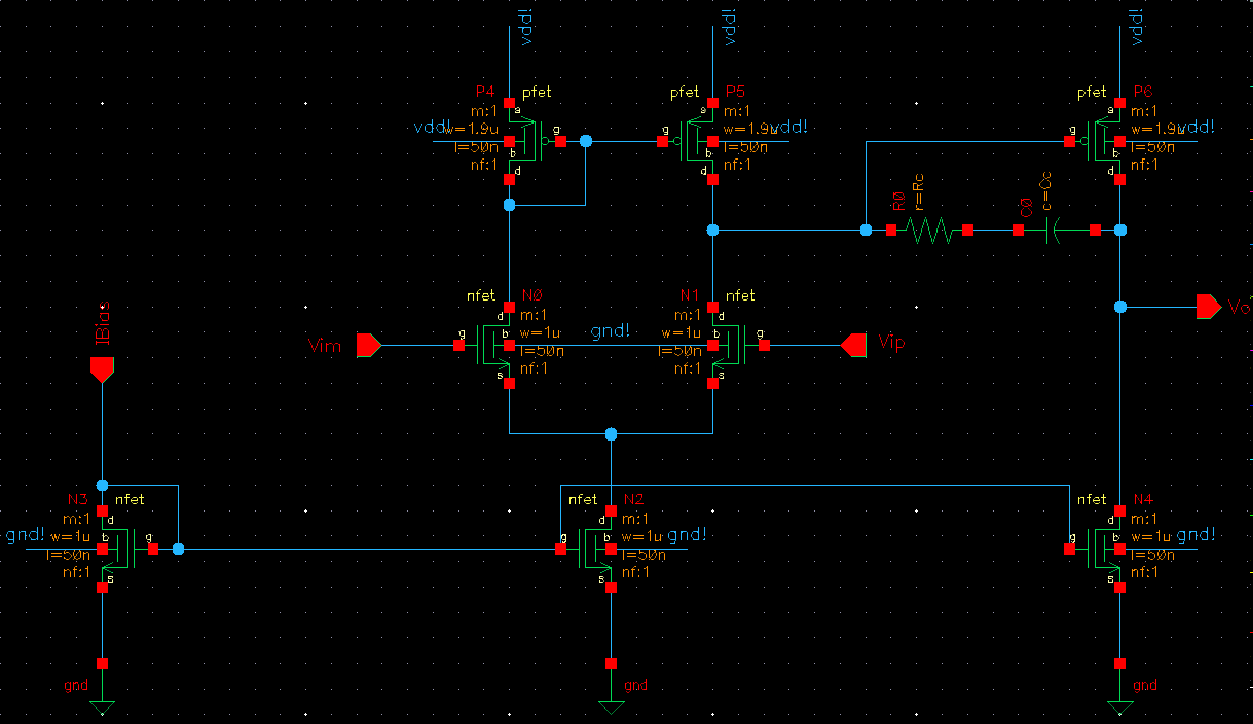
\includegraphics[width=\textwidth]{Images/OPASCH.png}
    \caption{Two figures across columns using subfig.}
    \label{fig_sim}
\end{figure*}


% \begin{figure*}[t!]
%     \centering
%     \subfloat[Op Amp Schematic]{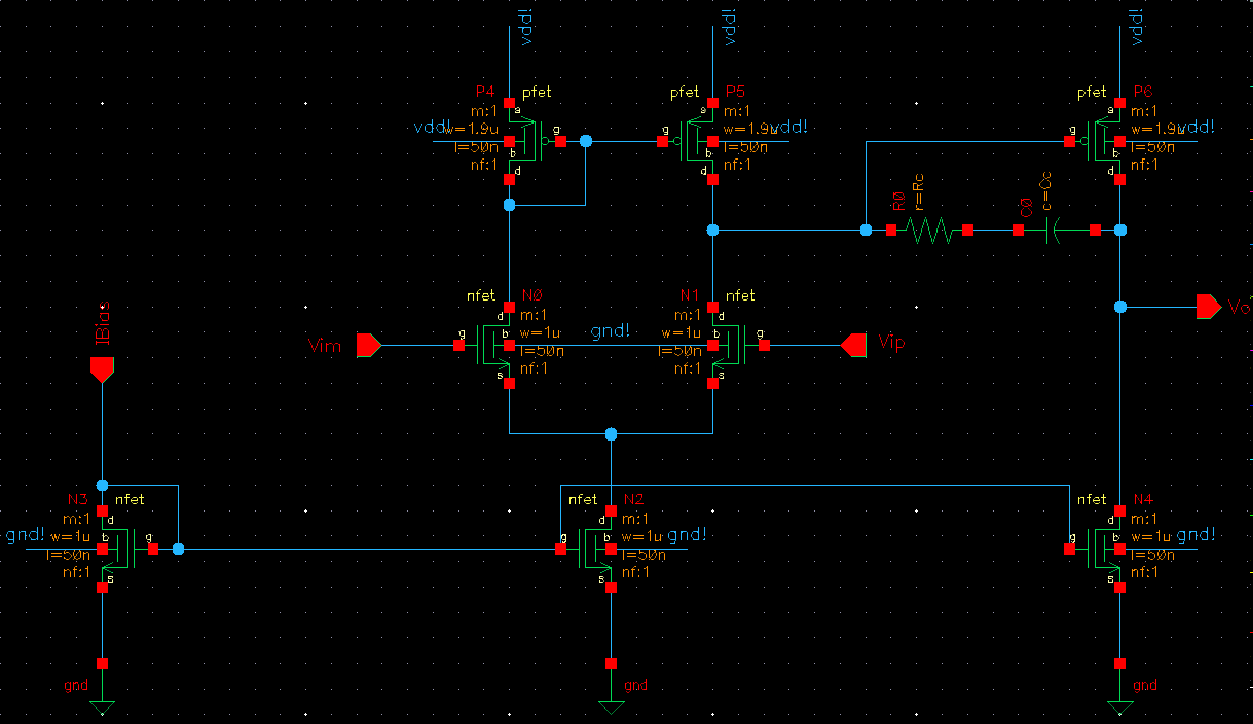
\includegraphics[width=3in]{Images/OPASCH.png}%
%     \label{fig_first_case}}
%     \hfil
%     \subfloat[I-V Curve]{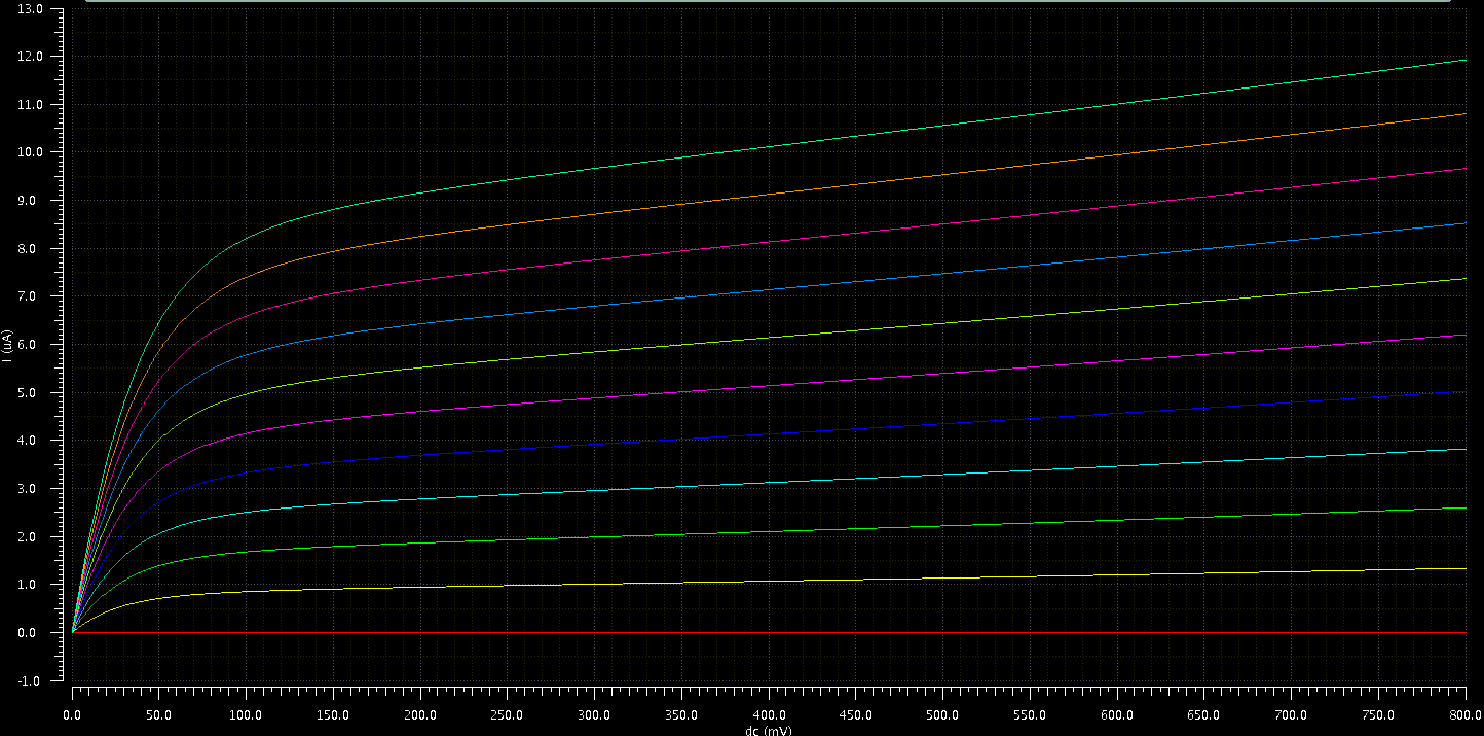
\includegraphics[width=3in]{Images/IVC.png}%
%     \label{fig_second_case}}
%     \caption{Two figures across columns using subfloat.}
%     \label{fig_sim}
% \end{figure*}

% \begin{figure*}[t!]
%     \centering
%     \subfigure[]{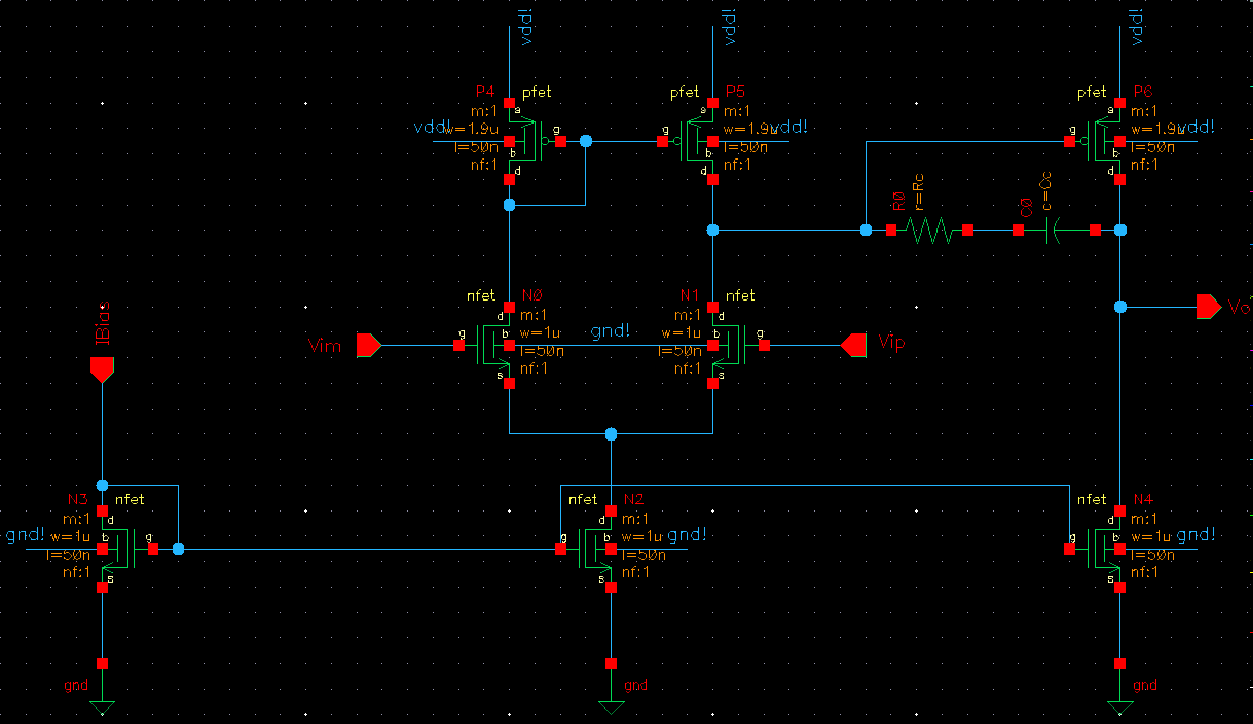
\includegraphics[width=3in]{Images/OPASCH.png}}
%     \subfigure[]{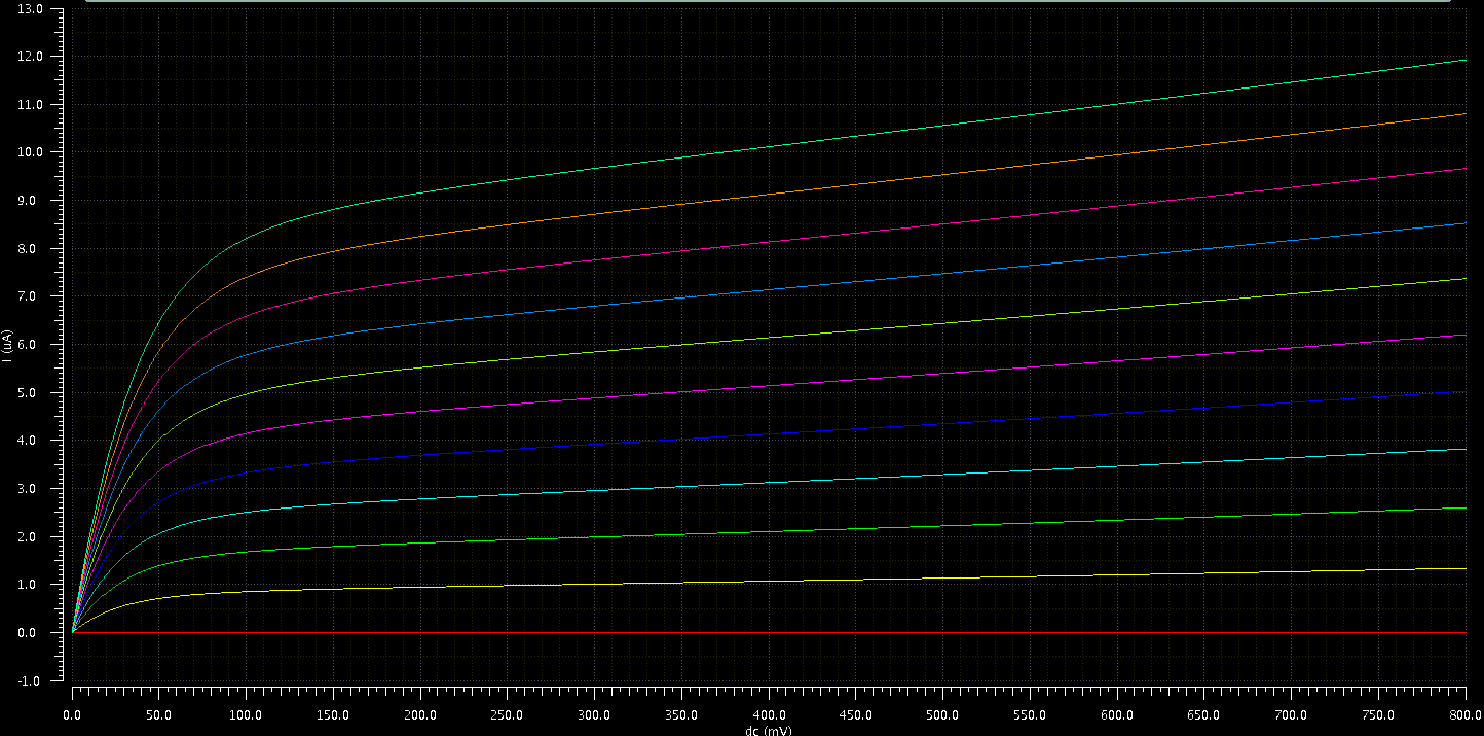
\includegraphics[width=3in]{Images/IVC.png}}
%     \caption{Two figures across columns using subfig.}
% \end{figure*}

    And example figure is given in figure \ref{dog_meme}. Whilst this figure may seem harmless, you must be sure to check the quality and resolution of your included figures. If the figures you place in your report are illegible, then it is not possible to award any marks for the work done (as it counts as no work done).

    Sometimes it may be difficult to get figures to behave and stay where you want them to on the page. This is where properties such as h! will assist you. You may also have figures float to the top (t!), which is very common in journal publications, however, it is not recommend in this context.

\subsection{Lab Equipment Specific Advice}
    This is for all that use lab equipment (looking at you 3106). Honestly, the best possible option is to save the data as a comma separated values (CSV) file and then plot the data in Python. It is the best way, you can control the DPI, resolution, colours, labels, truncate the data, etc. A white background with strong colours is always a good option; saves ink if printed as well. Try and make any colour pallet chosen compatible with black and white printers.
    
    If one does not wish to plot the data in Python/MATLAB, then a scope screenshot should suffice. Do not take pictures with your mobile phone, they are objectively bad. Also, crop the screenshots appropriately. For example, most of the time you do not need to see the information to the right of the waveform display.
    
\subsection{Cadence Virtuoso Specific Advice}

    Cadence is a complex electronic design automation (EDA) software. This complex nature causes labels and data points to not scale with window size. This would mean that if you were to screenshot a full screen window size plot, the data points will be so small that it will be hard for the reader to view.

\textbf{TIP:} To take good screenshots of a circuitry 
\begin{enumerate}
    \item Maximise the window.
    
    \item Press F to fit circuitry or layout to new window size.
    \item Take screenshot.
\end{enumerate}

    The plots presented in the figure below are nearly impossible to see. To avoid this, you can go into the Trace tab to change all plots to solid lines. Because Cadence is a complex software, you will have to apply this setting every time you wish to screenshot your plots. Red on black is hard to read, use bold brighter colours. 

\begin{figure}[h]
    \centering
    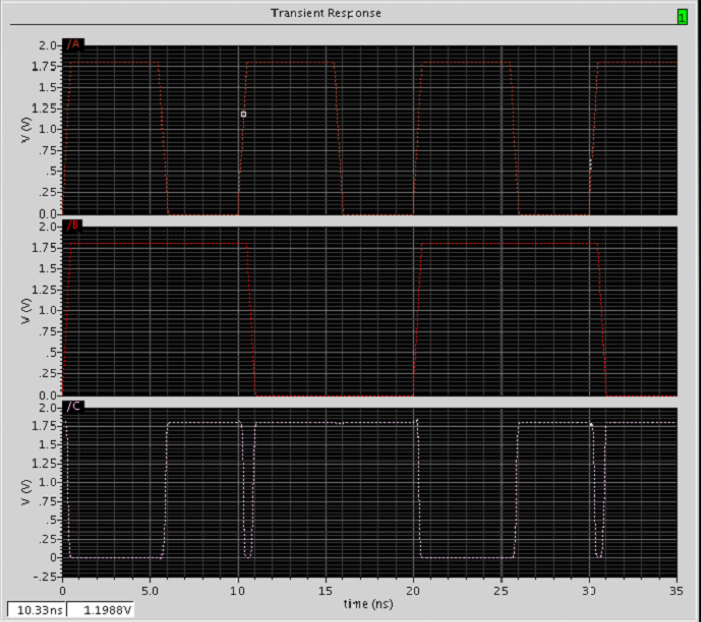
\includegraphics[width=2.5in]{Images/badplot.png}
    \caption{A bad figure.}
    \label{dog_meme}
\end{figure}

\newpage
\section{Tables}
    This is an example of a table. You can either directly edit the table in \LaTeX, however, there are multiple online and downloadable graphical editors that may make your life slightly easier.

\begin{table}[h!]
\renewcommand{\arraystretch}{1.3}
\caption{An Example of a Table}
\label{table_example}
\centering
\begin{tabular}{|c||c|}
    \hline
    One & Two\\
    \hline
    Three & Four\\
    \hline
\end{tabular}
\end{table}


\section{Double Stacked Figure}

    You can use a double stacked figure, however, you may run into issues as the template is designed for two separate columns. Typically this will cause the entire figure to appear on the second page. For best results you must have the floating option in a double stacked figure, as without this setting the figure may behave unpredictably. 

    You may also replace the two sub-floats with a single sub-float as this may be beneficial for landscape oriented images such as very large schematics or detailed plots.

    You may also notice that this image floats to the top of the page (as described before) so it may not be adjacent, or under a section heading and as such, care must be taken when in-text references are made. You should not be vague with wording (i.e. Do not use "The figure above", instead use "Figure 2"). And please, use symbolic links to figures, that way you never forget to label a figure (i.e. ``\textbackslash ref\{\}").

    In fact two examples are given, one utilising the subfig package and the other using subfloat. What you use is up to you. If you use either-or, please remove the unused package as you can see it causes conflicts and should never be used together, this is evident with the double parentheses around the subfig captions in figure \ref{fig_sim}.

\section{Conclusion}
    You should probably always place in a small conclusion to summaries your report.

    A few things to keep in mind:
\begin{itemize}
    \item A report is to convey observed information to the readers. Limit the use of vague words (Essentially, approximately, effectively etc.)
    \item Caption your figures. Label your tables. 
    \item Write you and your partner’s name and student ID or marks will not be inserted correctly.
    \item Explain your design decision. Use equations to support your observations. 
    \item If any experiment fails or did not meet expectation, document what happened and provide your thinking to why it may happen.
\end{itemize}

\section{References}
\printbibliography

\end{document}